
\documentclass{beamer}
\usecolortheme{dove}
\setbeamertemplate{navigation symbols}{}
\usepackage{amsmath,amssymb,amsfonts,amsthm, multicol, subfigure, color}
\usepackage{bm}
\usepackage{graphicx}
\usepackage{tabularx}
\usepackage{booktabs}
\usepackage{hyperref}
\usepackage{pdfpages}
\usepackage{xcolor}
\definecolor{seagreen}{RGB}{46, 139, 87}
\def\independenT#1#2{\mathrel{\rlap{$#1#2$}\mkern2mu{#1#2}}}
\newcommand\indep{\protect\mathpalette{\protect\independenT}{\perp}}
\def\log{\text{log}}
\newcommand\logit{\text{logit}}
\newcommand\iid{\stackrel{\text{iid}}{\sim}}
\newcommand\E{\text{E}}
\newcommand\V{\text{V}}
\renewcommand\P{\text{P}}
\newcommand{\Cov}{\text{Cov}}
\newcommand{\Cor}{\text{Cor}}
\newcommand\doop{\texttt{do}}
\usepackage{stackrel}
\usepackage{tikz}
\usetikzlibrary{arrows,shapes.arrows,positioning,shapes,patterns,calc}
\newcommand\slideref[1]{\vskip .1cm \tiny \textcolor{gray}{{#1}}}
\newcommand\red[1]{\color{red}#1}
\newcommand\blue[1]{\color{blue}#1}
\newcommand\gray[1]{\color{gray}#1}
\newcommand\seagreen[1]{\color{seagreen}#1}
\newcommand\purple[1]{\color{purple}#1}
\newcommand\orange[1]{\color{orange}#1}
\newcommand\black[1]{\color{black}#1}
\newcommand\white[1]{\color{white}#1}
\newcommand\teal[1]{\color{teal}#1}
\newcommand\magenta[1]{\color{magenta}#1}
\newcommand\Fuchsia[1]{\color{Fuchsia}#1}
\newcommand\BlueGreen[1]{\color{BlueGreen}#1}
\newcommand\bblue[1]{\textcolor{blue}{\textbf{#1}}}
\newcommand\bred[1]{\textcolor{red}{\textbf{#1}}}
\newcommand\bgray[1]{\textcolor{gray}{\textbf{#1}}}
\newcommand\bgreen[1]{\textcolor{seagreen}{\textbf{#1}}}
\newcommand\bref[2]{\href{#1}{\color{blue}{#2}}}
\colorlet{lightgray}{gray!40}
\pgfdeclarelayer{bg}    % declare background layer for tikz
\pgfsetlayers{bg,main} % order layers for tikz
\newcommand\mycite[1]{\begin{scriptsize}\textcolor{darkgray}{(#1)}\end{scriptsize}}
\newcommand{\tcframe}{\frame{
%\small{
\only<1|handout:0>{\tableofcontents}
\only<2|handout:1>{\tableofcontents[currentsection]}}
%}
}

\usepackage[round]{natbib}
\bibliographystyle{humannat-mod}
\setbeamertemplate{enumerate items}[default]
\usepackage{mathtools}

\newcommand{\goalsframe}{\begin{frame}{Learning goals for today}
At the end of class, you will be able to:
\begin{enumerate}
\item Estimate causal effects by outcome modeling with the parametric g-formula
\item See how this generalizes a common use of regression
\end{enumerate} \vskip .2in
\end{frame}}

\title{8. Parametric g-formula: Categorical treatments}
\author{Ian Lundberg\\Cornell Info 6751: Causal Inference in Observational Settings\\Fall 2022}
\date{15 Sep 2022}

\begin{document}

\maketitle

\goalsframe

\begin{frame}{Recap: Nonparametric identification} \pause

Three key assumptions: \vskip .2in
\begin{center}
\begin{tabular}{ll}
Consistency & $Y_i = Y_i^{A_i}$ \\
Exchangeability & $A\indep \{Y^a\}\mid \vec{L}$ \\
Positivity & $\P(A = a\mid \vec{L} = \vec\ell) > 0$
\end{tabular}
\end{center} \pause
These assumptions yield \bblue{nonparametric identification:}\\
a consistent estimator exists using observable sample means

\end{frame}

\begin{frame}{Recap: Nonparametric identification in a proof} \pause

$$\begin{aligned}
\E(Y^a) \pause &= \sum_{\vec\ell}\P(\vec{L} = \vec\ell) \E(Y^a\mid \vec{L} = \vec\ell) &\text{rules of probability} \\ \pause
&=  \sum_{\vec\ell}\P(\vec{L} = \vec\ell) \E(Y^a\mid \vec{L} = \vec\ell, A = a) &\text{exchangeability} \\ \pause
&= \sum_{\vec\ell}\P(\vec{L} = \vec\ell) \E(Y\mid \vec{L} = \vec\ell, A = a) &\text{consistency} \pause
\end{aligned}$$

Positivity ensures $\E(Y\mid \vec{L} = \vec\ell, A = a)$ can be estimated from data. \vskip .2in \pause
\bgray{What we gained}: In an infinite sample, we can estimate causal effects by taking means and aggregating!

\end{frame}

\begin{frame}{Recap: Nonparametric identification with two Es}

For simplicity, rewrite the previous result with two expectations \pause

$$\begin{aligned}
\E(Y^a) &= \sum_{\vec\ell}\P(\vec{L} = \vec\ell) \E(Y\mid \vec{L} = \vec\ell, A = a) \\ \pause
&= \E\bigg(\E(Y\mid \vec{L}, A = a)\bigg)
\end{aligned}$$ \pause
There are two pieces \pause
\begin{itemize}
\item Inner expectation: Within groups
\begin{itemize}
\item Mean over units within each stratum of confounders
\end{itemize} \pause
\item Outer expectation: Across groups
\begin{itemize}
\item Mean of that over the population distribution of $\vec{L}$
\end{itemize}
\end{itemize}

\end{frame}

\begin{frame}{Recap: Nonparametric identification. An estimator}

Nonparametric identification yielded this estimand:
$$\E(Y^a) = \E\bigg(\E(Y\mid \vec{L}, A = a)\bigg)$$ \pause
This points toward a \bblue{non-parametric plug-in estimator}: \pause
\begin{itemize}
\item Inner expectation: Sample mean in each subgroup \pause
\item Outer expectation: Mean over full sample
\end{itemize} \pause \vskip .1in
Resulting estimator:
$$\begin{aligned}
\hat\E(Y^a) &= \frac{1}{n}\sum_{i=1}^n \hat\E(Y\mid \vec{L} = \vec\ell_i, A = a)
\end{aligned}$$
\end{frame}

\begin{frame}{Recap: Nonparametric identification. An estimator}
Putting this in words:
$$\begin{aligned}
\hat\E(Y^a) &= \frac{1}{n}\sum_{i=1}^n \hat\E(Y\mid \vec{L} = \vec\ell_i, A = a)
\end{aligned}$$
\begin{itemize}
\item Sample average over units $i$
\item For each unit, take the sample average outcome among
\begin{itemize}
\item Units with their covariate values $\vec\ell_i$
\item But who have the relevant treatment value $A = a$
\end{itemize}
\end{itemize}
It is all just sample means, aggregated a certain way.

\end{frame}

\begin{frame}{Why move to \bblue{parametric} estimation?} \pause

Some reasons for a parametric model: \pause
\begin{enumerate} \pause
\item \bgray{Empty cells:} Despite positivity in the population, some sample strata have no units with $A = a$. Nonparametric estimation is impossible \pause
\item \bgray{Continuous confounders:} If any variables in $\vec{L}$ are continuous, then each stratum of $\vec{L}$ contains only one unit. Empty cells are inevitable \pause
\item \bgray{Estimation variance:} Even if you can do nonparametric estimation, it involves estimating numerous means. This may be a high-variance approach, resulting in extensive statistical uncertainty
\end{enumerate}

\end{frame}

\begin{frame}{The parametric g-formula} \pause

Nonparametric identification yielded this estimand:
$$\E(Y^a) = \E\bigg(\E(Y\mid \vec{L}, A = a)\bigg)$$ \pause
What if we estimated $\E(Y\mid \vec{L} = \vec\ell, A = a)$ with a regression model?
\end{frame}

\begin{frame}{The parametric g-formula: Simple case}

\begin{center}
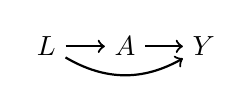
\begin{tikzpicture}
\node (l) at (0,0) {$L$};
\node (a) at (1,0) {$A$};
\node (y) at (2,0) {$Y$};
\draw[->, thick] (l) -- (a);
\draw[->, thick] (a) -- (y);
\draw[->, thick] (l) to[bend right] (y);
\end{tikzpicture}
\end{center} \pause
\begin{tabular}{ll}
Nonparametric identification & $\E(Y^a) = \E(\E(Y\mid L, A = a))$ \\ \pause
\\
Parametric model & $\E(Y\mid L, A) = \alpha + \gamma L + \beta A$
\end{tabular} \vskip .1in \pause
Estimator for the potential outcome under treatment ($A = 1$):
$$\hat\E(Y^1) = \frac{1}{n}\sum_{i=1}^n \bigg(\hat\alpha + \hat\gamma \ell_i + \hat\beta \times 1\bigg)$$ \pause
Estimator in words:
\begin{enumerate} \pause
\item Estimate the regression model \pause
\item Change all treatment values to 1 \pause
\item Predict for everyone \pause
\item Take the sample mean
\end{enumerate}

\end{frame}

\begin{frame}{The parametric g-formula: Connection to $\hat\beta$} \pause
Estimator for the effect $\E(Y^1) - \E(Y^0)$: \pause
$$\begin{aligned}
\hat\E(Y^1) - \hat\E(Y^0)  \pause
&= \left(\frac{1}{n}\sum_{i=1}^n \bigg(\hat\alpha + \hat\gamma \ell_i + \hat\beta \times 1\bigg)\right) \\ \pause
&\qquad - \left(\frac{1}{n}\sum_{i=1}^n \bigg(\hat\alpha + \hat\gamma \ell_i + \hat\beta \times 0\bigg)\right) \\ \pause
&= \frac{1}{n}\sum_{i=1}^n \hat\beta \\ \pause
&= \hat\beta
\end{aligned}$$ \pause
With OLS, the parametric g-formula collapses on the coefficient.
\end{frame}

\begin{frame}{The parametric g-formula is more general} \pause
Suppose we add the $A\times L$ interaction to the model.
$$\E(Y\mid A, L) = \alpha + \gamma L + \beta A + \eta AL$$ \pause
Estimator for the effect $\E(Y^1) - \E(Y^0)$: \pause
$$\begin{aligned}
\hat\E(Y^1) - \hat\E(Y^0)  \pause
&= \left(\frac{1}{n}\sum_{i=1}^n \bigg(\hat\alpha + \hat\gamma \ell_i + \hat\beta \times 1 + \hat\eta \times  1\times \ell_i)\bigg) \right) \\ \pause
&\qquad - \left(\frac{1}{n}\sum_{i=1}^n \bigg(\hat\alpha + \hat\gamma \ell_i + \hat\beta \times 0 + \hat\eta\times 0 \times \ell_i\bigg) \right) \\ \pause
&= \frac{1}{n}\sum_{i=1}^n \left(\hat\beta + \hat\eta \ell_i\right) \pause
\end{aligned}$$
The g-formula no longer collapses to a coefficient!
\end{frame}

\begin{frame}{The parametric g-formula: Word of warning} \pause

The parametric g-formula does not replace any assumptions.\vskip .2in \pause
You need:
\begin{center}
\begin{tabular}{ll}
\multicolumn{2}{l}{\bgray{Identification Assumptions (causal)}} \\
Consistency & $Y_i = Y_i^{A_i}$ \\
Exchangeability & $A\indep \{Y^a\}\mid \vec{L}$ \\
Positivity & $\P(A = a\mid \vec{L} = \vec\ell) > 0$ \\
{} \\
\multicolumn{2}{l}{\bgray{Estimation Assumptions (statistical)}} \\
Estimation & $\E(Y\mid A, \vec{L})$ follows the assumed model
\end{tabular}
\end{center} \pause
To use a parametric model, we \bgray{added} the bottom assumption. \pause
\begin{itemize}
\item But testable! Diagnostics and out-of-sample performance
\end{itemize}

\end{frame}

\begin{frame}{The parametric g-formula: Summary}

\begin{center} \pause
The parametric g-formula is how we answer\\nonparametric causal questions\\with\\parametric outcome modeling tools
\end{center} \vskip .1in
\begin{itemize} \pause
\item Allows you to use a model for $\E(Y\mid A, \vec{L})$ \pause
\item The model is exactly as in standard non-causal statistics \pause
\item The estimator is operationalized by prediction: \pause
\begin{itemize}
\item Estimate the regression \pause
\item Modify the treatment \pause
\item Make new predictions \pause
\item Average over the sample
\end{itemize}
\end{itemize}

\end{frame}


\goalsframe

\begin{frame}{Let me know what you are thinking}

\begin{huge} \bref{https://tinyurl.com/CausalQuestions}{tinyurl.com/CausalQuestions} \end{huge}
\vskip .7in

Office hours TTh 11am-12pm and at \bref{https://calendly.com/ianlundberg/office-hours}{calendly.com/ianlundberg/office-hours}\\Come say hi!

\end{frame}

\end{document}

